\documentclass[12pt, a4paper]{article}
\usepackage{ctex}
\usepackage{amsmath,amscd,amsbsy,amssymb,latexsym,url,bm,amsthm}
\usepackage{caption}
\usepackage{epsfig,graphicx,subfigure}
\usepackage{enumitem,balance}
\usepackage{wrapfig}
\usepackage{listings}
\usepackage{mathrsfs,euscript}
\usepackage[usenames]{xcolor}
\usepackage{hyperref}
\usepackage[vlined,ruled,linesnumbered]{algorithm2e}
\hypersetup{colorlinks=true,linkcolor=black}

\captionsetup[figure]{
	labelfont = {bf},
	labelformat = {default},
	labelsep = period,
	name = {Fig.}
}

\newtheorem{theorem}{Theorem}
\newtheorem{lemma}[theorem]{Lemma}
\newtheorem{proposition}[theorem]{Proposition}
\newtheorem{corollary}[theorem]{Corollary}
\newtheorem{exercise}{Exercise}
\newtheorem*{solution}{Solution}
\newtheorem{definition}{Definition}
\theoremstyle{definition}
\lstset{
	keywordstyle = \color{blue!70}\bfseries, 
	basicstyle = \ttfamily, 
	commentstyle = \ttfamily,
	showstringspaces = false,
	frame = shadowbox,
	rulesepcolor = \color{red!20!green!20!blue!20},
}

\renewcommand{\thefootnote}{\fnsymbol{footnote}}

\newcommand{\postscript}[2]{
	\setlength{\epsfxsize}{#2\hsize}
  	\centerline{\epsfbox{#1}}
}

\renewcommand{\baselinestretch}{1.0}

\setlength{\oddsidemargin}{-0.35in}
\setlength{\evensidemargin}{-0.35in}
\setlength{\topmargin}{-0.3in}
\setlength{\headheight}{0in}
\setlength{\headsep}{0in}
\setlength{\textheight}{10.2in}
\setlength{\textwidth}{7in}
\makeatletter 
\renewenvironment{proof}[1][Proof] {\par\pushQED{\qed}\normalfont\topsep6\p@\@plus6\p@\relax\trivlist\item[\hskip\labelsep\bfseries#1\@addpunct{.}]\ignorespaces}{\popQED\endtrivlist\@endpefalse} \makeatother
\makeatletter
\renewenvironment{solution}[1][Solution] {\par\pushQED{\qed}\normalfont\topsep6\p@\@plus6\p@\relax\trivlist\item[\hskip\labelsep\bfseries#1\@addpunct{.}]\ignorespaces}{\popQED\endtrivlist\@endpefalse} \makeatother

\begin{document}
\noindent

%========================================================================
\noindent\framebox[\linewidth]{\shortstack[c]{
\Large{\textbf{Lab \#1: Measurement of WiFi Signal Strength}}\vspace{1mm}\\
EE447 Mobile Network, Luoyi Fu, Spring 2021\\
\textbf{Due}: \textit{Sunday, Apr 18th}}}
\begin{center}

Name: Hongjie Fang  \quad Student ID:518030910150 \quad Email: \href{mailto:galaxies@sjtu.edu.cn}{galaxies@sjtu.edu.cn}
\end{center}

\section{Purpose and Objective}\label{section1}
This lab aims to let us get used to the WiFi system, and accomplish the sampling and measuring of WiFi signal strength through programming in Android on smartphone. 

In other words, we are going to design a positioning Android application based on Wifi signal strength, in which we will implement an effective algorithm for indoor positioning using the signal strength data of WiFi sensor in the mobile phone.

\section{Indoor Positioning Algorithm}\label{section2}
Our approach is based on the idea that the signal strength has a relationship with the distance between the router and the smartphone. From the textbook and other materials, we can find out that they follows the following equation.

$$
d = 10^{\frac{|RSSI| - A}{10n}}
$$

\noindent where $A$ is the power value in the position which is 1m to the router,  $n$ is the path loss coefficient, and $RSSI$ is the signal strength of WiFi router. Both $A$ and $n$ is determined by the experiment environment and the type of the router. Thus we can set them fixed in the equation. Since $RSSI$ is usually negative and increases as the power increases, \textit{i.e.}, $RSSI$ increases as the distance decreases, we take absolute value of $RSSI$ in the previous equation, which is quite reasonable.

Suppose we have $n$ WiFi routers, namely $R_1, R_2, \cdots, R_n$. Suppose the $i$-th WiFi router $R_i$ is located in $(x_i, y_i)$ in the coordinate system, which can be measured priorly. We can measure the distance $d_i$ between the smartphone and the $i$-th WiFi router $R_i$ using the previous equation. Intuitively, the position of smartphone $(x, y)$ should meet the following requirements.

$$
(x - x_i)^2 + (y - y_i)^2 = d_i^2\quad \quad (i=1,2,\cdots, n)
$$

Unfortunately, due to the precison and accuracy reasons of both WiFi signal strength and WiFi router locations, this equation may not have a solution when $n \ge 3$, \textit{i.e.}, when additional requirements are setted. Therefore, we are going to use machine learning methods to calculate the position $(x,y)$ of smartphone. More formally, if the current estimate position of the smartphone is $(x, y)$, then we can define the \textbf{loss function} of the current estimators as follows.

$$
\mathcal{L}(x, y) = \frac{1}{n}\sum_{i=1}^n\left((x - x_i)^2 + (y - y_i)^2 - d_i^2\right)^2
$$

\noindent which is the typical square loss function. Hence, we can transform our problem into the following optimization problem.

$$
\begin{aligned}
&&\min_{x,y} &\quad \mathcal{L}(x, y) \\
&&\textrm{s.t.} &\quad (x,y) \in \mathbb{E}
\end{aligned}
$$

\noindent where $\mathbb{E}$ is the feasible space of the smartphone. In experimental setup, we can regard $\mathbb{E}$ as $\mathbb{R}^2$, \textit{i.e.}, the smartphone can locate in any place in the experimental space.

Therefore, we can use \textbf{Gradient Descent Algorithm} to solve the optimization problem. More specifically, we can first derive the gradient of the loss function as follows.

$$
\begin{aligned}
&\frac{\partial \mathcal{L}(x, y)}{\partial x} = \frac{1}{n} \sum_{i=1}^n\frac{\partial}{\partial x}\left((x - x_i)^2 + (y - y_i)^2 - d_i^2\right)^2 = \frac{4}{n}\sum_{i=1}^n ((x-x_i)^3-d_i^2(x-x_i)+(y-y_i)^2(x-x_i)) \\
&\frac{\partial \mathcal{L}(x, y)}{\partial y} = \frac{1}{n} \sum_{i=1}^n\frac{\partial}{\partial y}\left((x - x_i)^2 + (y - y_i)^2 - d_i^2\right)^2 = \frac{4}{n}\sum_{i=1}^n ((y-y_i)^3-d_i^2(y-y_i)+(x-x_i)^2(y-y_i))
\end{aligned}
$$

Hence, let $(\hat{x}_t,\hat{y}_t)$ denote the current estimate position of the smartphone, we can update the estimators $(\hat{x}_{t+1}, \hat{y}_{t+1})$ as follows.

$$
\begin{aligned}
&\hat{x}_{t+1} = \hat{x}_t - \eta_t \left.\frac{\partial \mathcal{L}(x, y)}{\partial x}\right|_{x = \hat{x}_t} = \hat{x}_t - \frac{4\eta_t}{n}\sum_{i=1}^n ((\hat{x}_t-x_i)^3-d_i^2(\hat{x}_t-x_i)+(\hat{y}_t-y_i)^2(\hat{x}_t-x_i))\\
&\hat{y}_{t+1} = \hat{y}_t - \eta_t \left.\frac{\partial \mathcal{L}(x, y)}{\partial x}\right|_{y = \hat{y}_t} = \hat{y}_t - \frac{4\eta_t}{n}\sum_{i=1}^n ((\hat{y}_t-y_i)^3-d_i^2(\hat{y}_t-y_i)+(\hat{x}_t-x_i)^2(\hat{y}_t-y_i))
\end{aligned}
$$

\noindent where $\eta_t$ is the learning rate in the $t$-th iteration.

Thus, we continue updating the position estimators $(\hat{x}, \hat{y})$ until the process converges, \textit{i.e.},

$$
\left|\mathcal{L}(\hat{x}_{t+1}, \hat{y}_{t+1}) - \mathcal{L}(\hat{x}_t, \hat{y}_t)\right| < \varepsilon
$$
\noindent where $\varepsilon$ is the thershold and is usually set as $10^{-8}$.

In conclusion, our indoor positioning algorithm is based on the relationship between the distance and the signal strength, and we form the problem as an optimization problem and apply Gradient Descent Algorithm to solve it.

\section{Implementation}\label{section3}
\subsection{Given Codes}\label{section3.1}
We are given some initial codes to complete the lab, so we should understand these codes first.

The initial codes has two Java classes, namely \texttt{MainActivity} and \texttt{SuperWiFi}, and the latter one is the extension of the first one. We focus on \texttt{MainActivity} first. It asks for the necessary permission and then shows the application layout, which contains two buttons \texttt{Scan}, \texttt{Clean} and a textbox. When pressing the \texttt{Scan} button, it will call methods in \texttt{SuperWiFi} class to scan for WiFi signals and calculate the $RSSI$, then it will print the result in the textbox. The main logic of the initial given application can be illustrated as follows.
\begin{figure}[htbp]
	\centering
	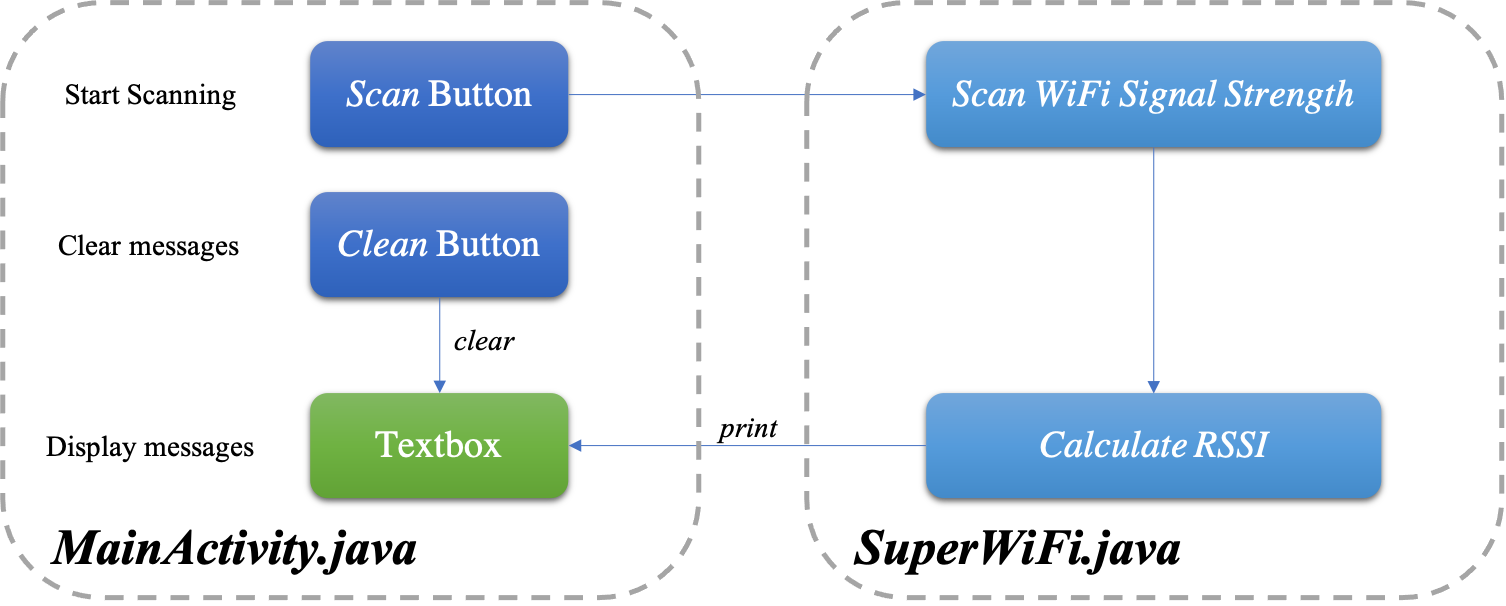
\includegraphics[width=4.2in]{1.png}
	\caption{The logic of the initial given application}
	\label{fig1}
\end{figure}

\subsection{My Implementations}\label{section3.2}
Some critical modifications are made to the original applications. First, we apply the algorithm introduced in Section \ref{section2} in \texttt{SuperWiFi} module to calculate the position of the smartphones. Here are some specific details of the experimental setup.
\begin{itemize}
	\item $A$, which is the power value in the position which is 1m to the router, is set to the average value of $60$;
	\item $n$, which is the path loss coefficient, is set to $3.25$ as usual;
	\item We use 4 Wi-Fi routers named \texttt{406}, \texttt{408}, \texttt{507}, \texttt{508} in the experiment, and their positions are $(-3.6, 0.4)$, $(4.5, -2.3)$, $(2.3, 1.9)$, $(3.2, -5.2)$ respectively;
	\item $\eta_t$, which is the learning rate, is set to $10^{-3}$ for all $t$;
	\item $\varepsilon$, which is the threshold, is set to $10^{-8}$ as usual.
\end{itemize}

Some implementation details are listed as follows.
\begin{itemize}
    \item First, we check the condition of all routers. If some routers are offline, their $RSSE$ value will be $0$ and we won't consider them in the following positioning process.
    \item Second, we calculate the $RSSE$ value of all valid routers. If the number of valid routers is less than $3$, then we do not perform positioning since the information is not enough to produce accurate positioning results.
    \item Then, we apply the algorithm introduced in Section \ref{section2} to perform positioning, which is shown in Appendix A.
    \item Finally, we calculate the necessary values for further visualization process, which is shown in Appendix A.
\end{itemize}

Apart from the previous modifications, we also add some features in the layout. We add a \texttt{Visualization} button to show the positioning result in a more intuitive way. Therefore, the main logic of my modified application can be illustrated as follows. 
\begin{figure}[htbp]
	\centering
	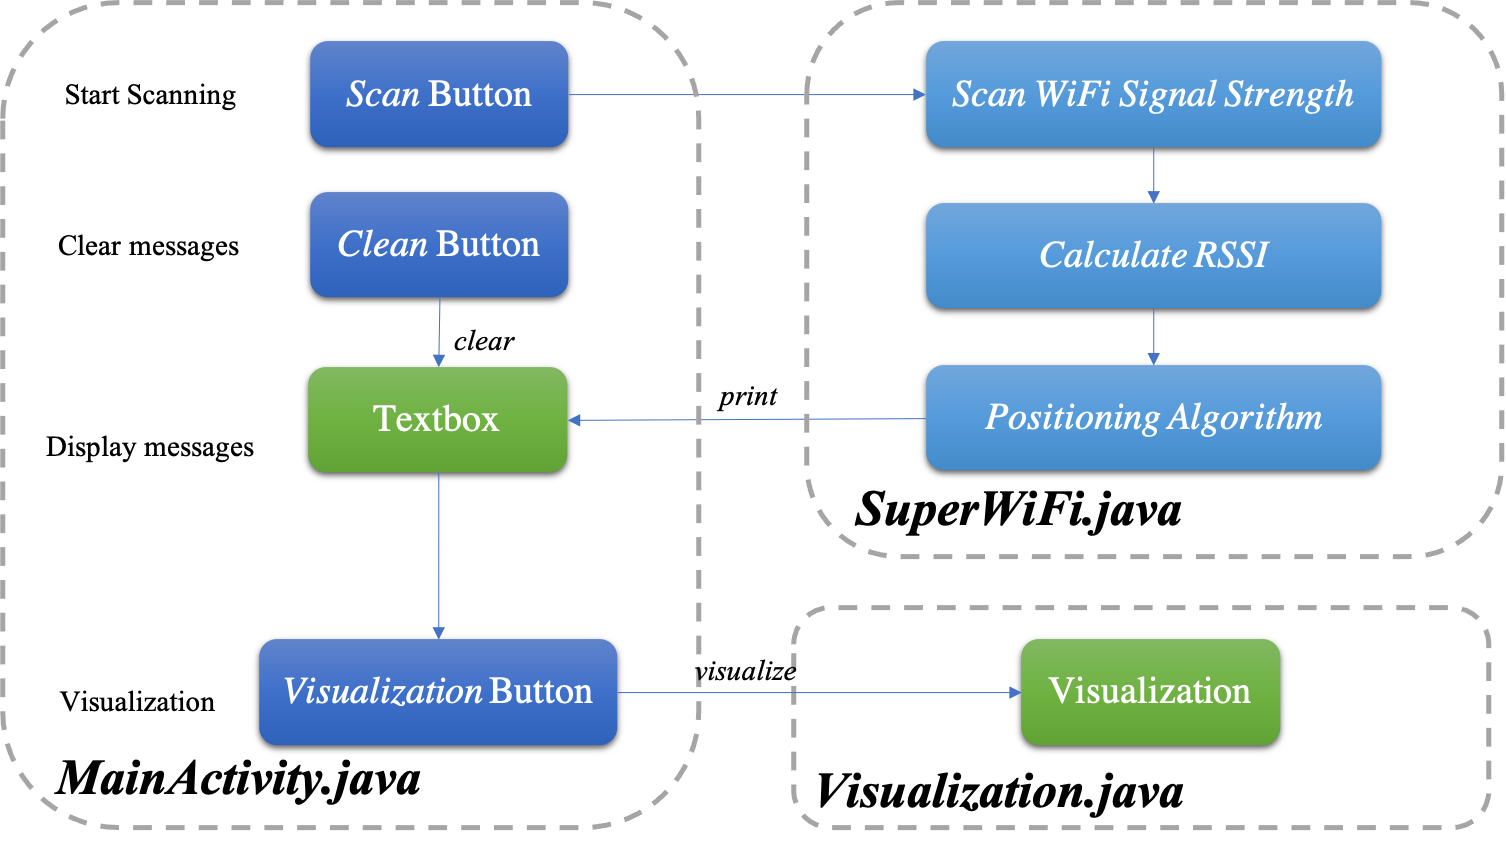
\includegraphics[width=4.2in]{2.png}
	\caption{The logic of my modified application}
	\label{fig2}
\end{figure}

We mainly use \texttt{Canvas} package in Java for visualization, and the effect of visualization will be illustrated later in Section \ref{section4}

\section{Experiments}\label{section4}
We use Huawei P20 smartphone in real-world setup testing. The experimental results are shown in Fig. \ref{fig3} and Fig. \ref{fig4}.

\begin{figure}[htbp]
	\begin{minipage}[t]{0.5\linewidth}
		\centering
		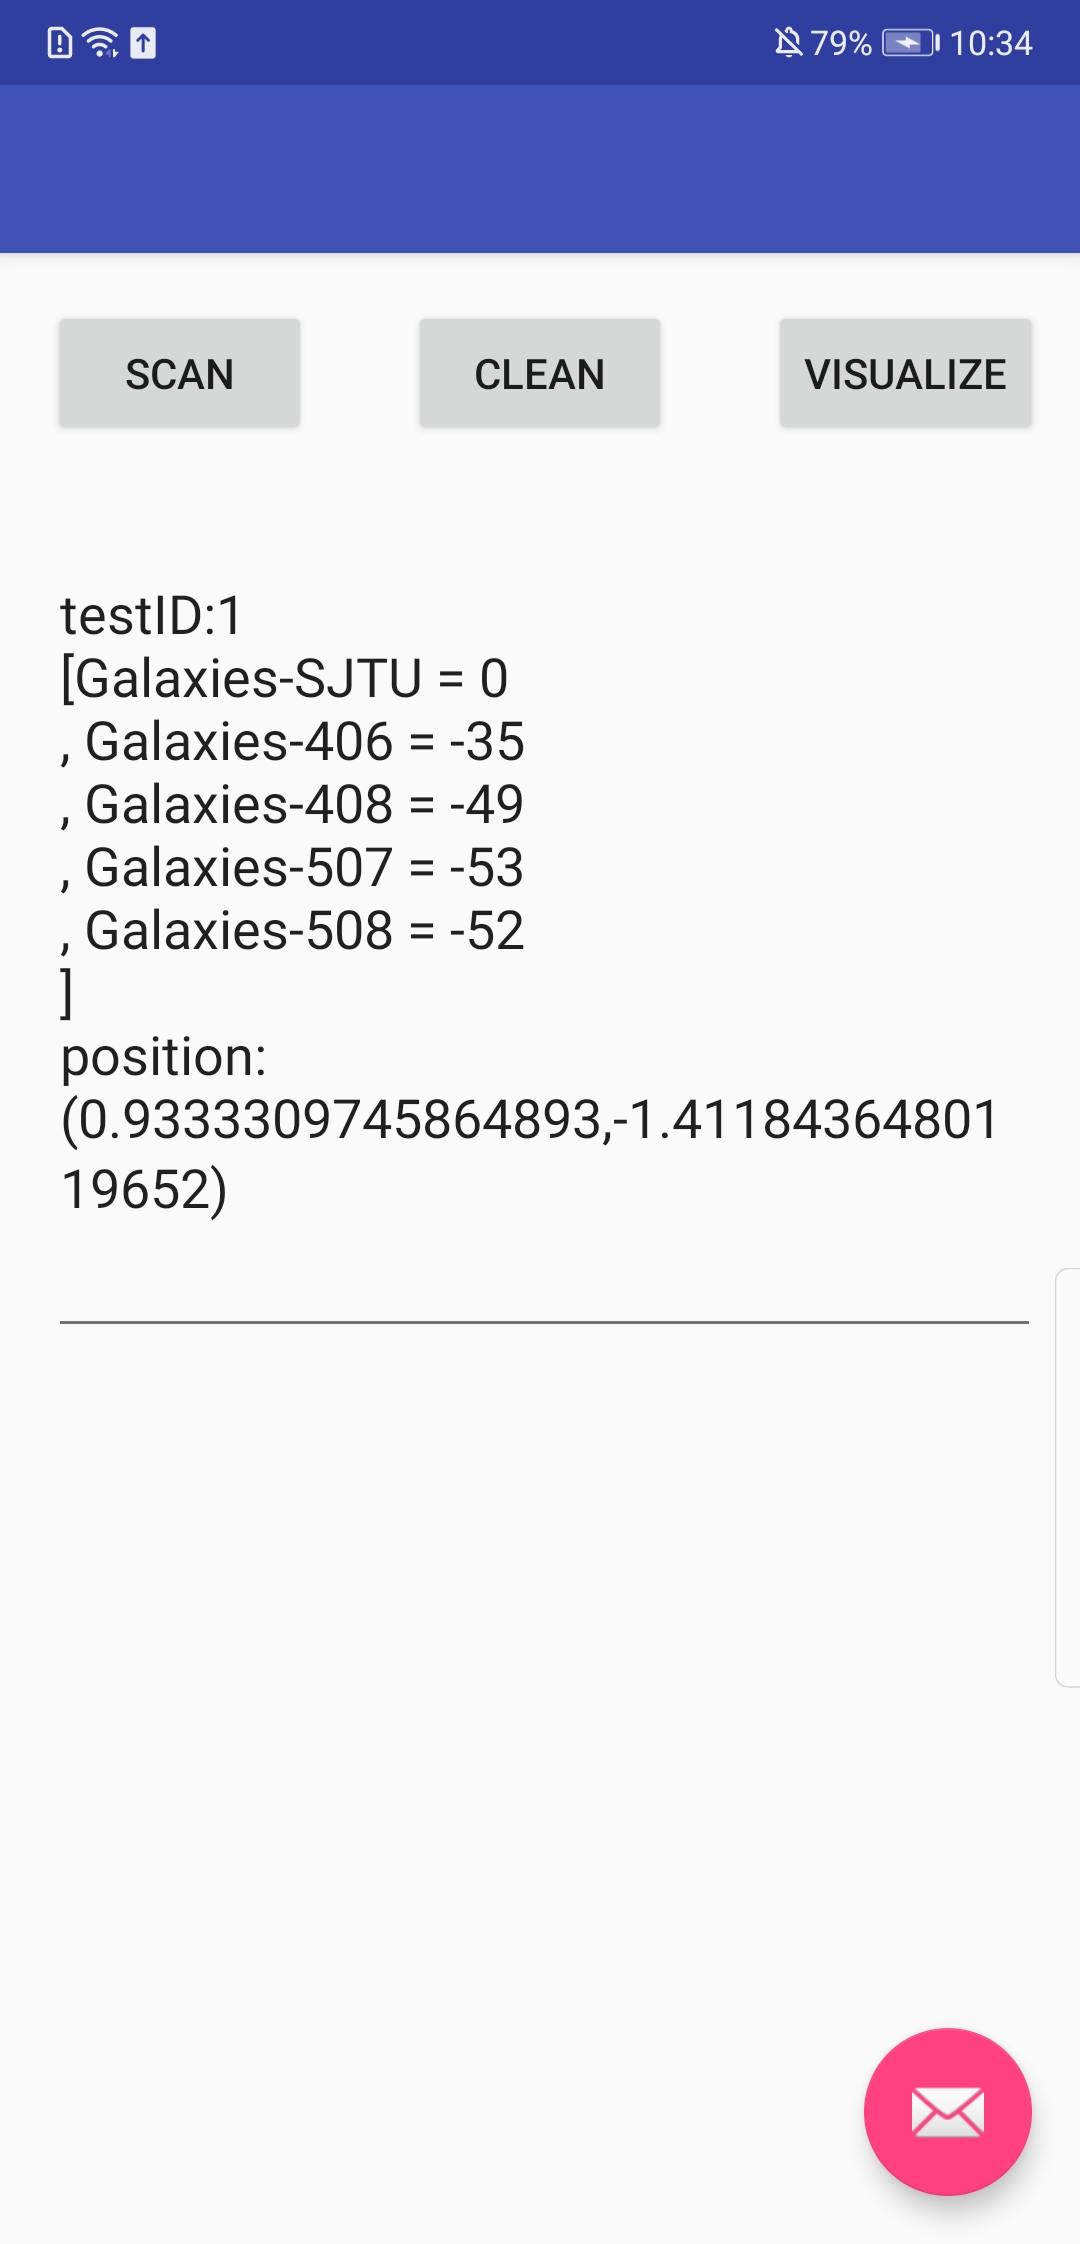
\includegraphics[width=2.3in]{3.jpeg}
		\caption{Experimental Results}
		\label{fig3}
		\end{minipage}%
		\begin{minipage}[t]{0.5\linewidth}
		\centering
		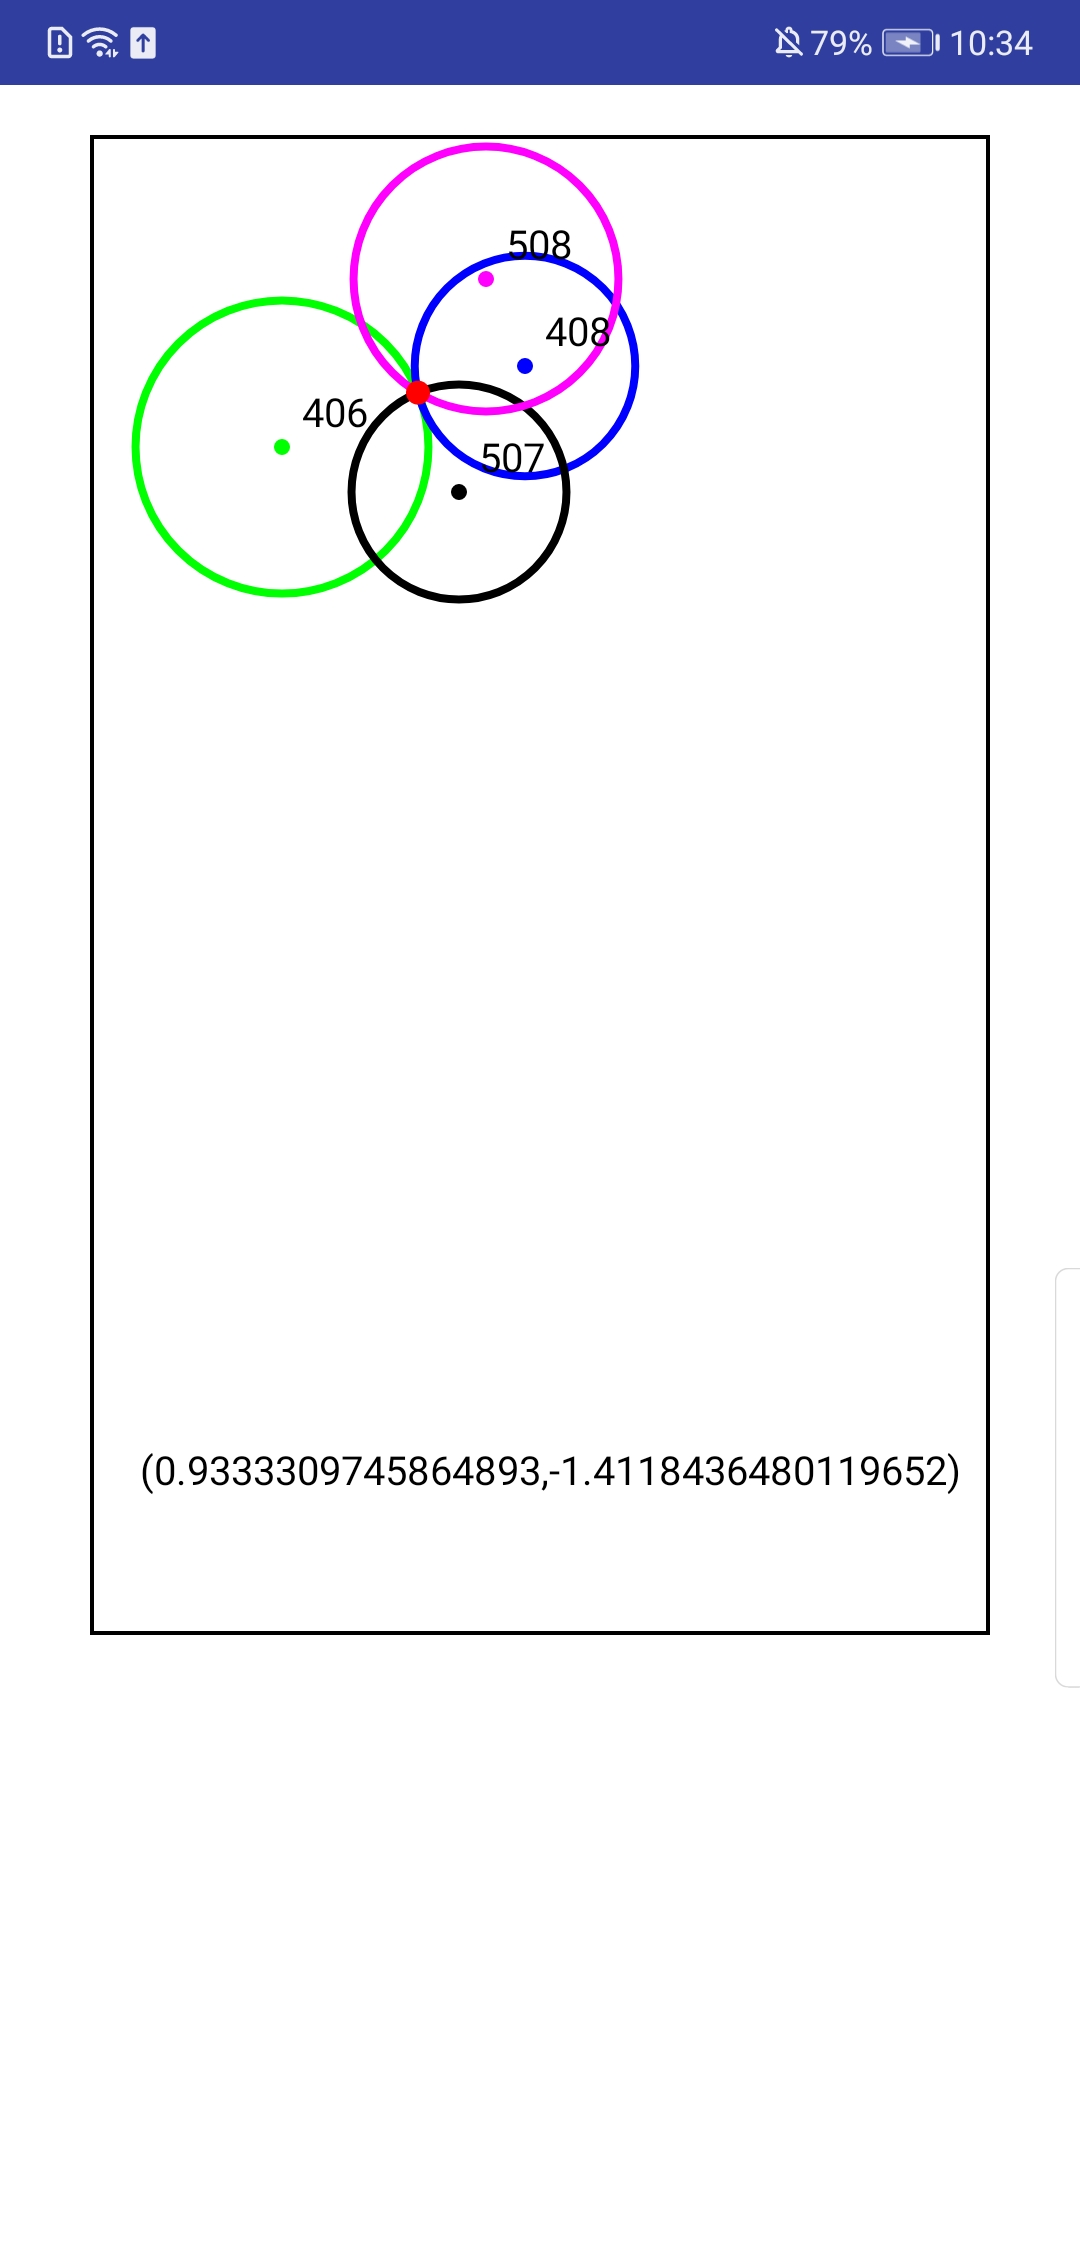
\includegraphics[width=2.3in]{4.jpeg}
		\caption{Visualizations}
		\label{fig4}
		\end{minipage}
\end{figure}

From Fig. \ref{fig3} we can see that the application detects the signal strength of all testing WiFis, and does not find the WiFi SJTU since it is not covered yet in the dormitory area. Use the four testing WiFis, we successfully calculate the position of the smartphone, and Fig. \ref{fig4} illustrates the relative position of the smartphone and the testing WiFis.

Therefore, our application completes all the required functions, and is able to perform positioning based on the WiFi signal strength of several testing WiFis.

\section{Questions and Answers}
\begin{enumerate}
\item \textbf{Q: Why is necessary to record all the measured value rather than only the average value? Please give your own explanation.}

\textbf{A: } If we only record average value of the strength of WiFi signals, we will lose some important information for debug. For example, during my debugging process, I once find that the scanning results seems incorrect. After checking all the records, I find that there are many outliers samples in the records, which may be caused by the distance between the WiFi and the smartphone is too far. When I choose another WiFi which is closer to the smartphone for testing, the results becomes reasonable. Therefore, I benifit a lot from the full records during debugging, and this is an important reason for recording all the measured value rather than only the average value.

\item \textbf{Q: Besides the WiFi signal strength, what other information of the Routers can be got in the test?}

\textbf{A: } After calling \texttt{WiFiManager.getScanResults()}, we can get a list of the scanning results shown as follows.

\begin{figure}[htbp]
	\centering
	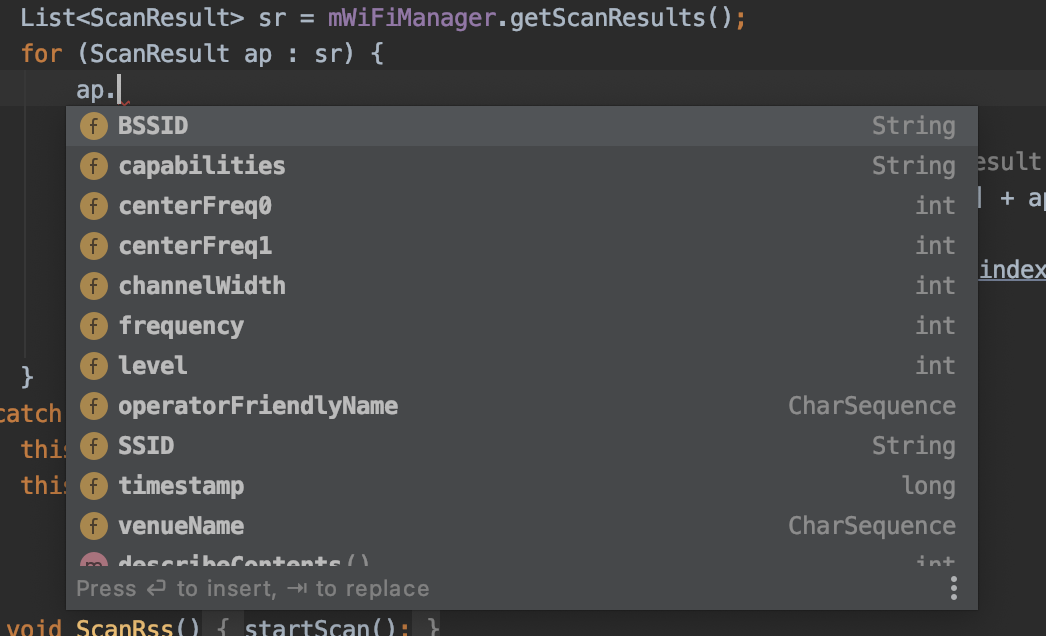
\includegraphics[width=4.2in]{5.png}
	\caption{The information contained in the \texttt{ScanResult}}
	\label{fig5}
\end{figure}

Here are some explanations for the information.

\begin{itemize}
\item \texttt{BSSID}: the address of the access point.
\item \texttt{capabilities}: describe the authentication schemes, encryption schemes and other schemes that is supported by the access point.
\item \texttt{centerFreq0}: center frequency (of the first segment) used if AP bandwidth is greater than $20 MHz$.
\item \texttt{centerFreq1}: center frequency of the second segment only used if AP bandwidth is $80 + 80 MHz$.
\item \texttt{channelWidth}: the channel width.
\item \texttt{frequency}: the primary frequency of the channel.
\item \texttt{level}: the detected signal strength level in the unit of \texttt{dBm}, \textit{a.k.a.}, $RSSI$.
\item \texttt{operatorFriendlyName}: passpoint operator name published by the access point.
\item \texttt{SSID}: the network name.
\item \texttt{timestamp}: the timestamp of the connection.
\item \texttt{venueName}: venue name published by the access point.
\end{itemize}

\item \textbf{Q: Why does the scanning need to be operated in thread ``scanThread''?}

\textbf{A: } I think the main reason is \textbf{efficiency}. Since the scanning process may take up lots of time, if we implement the scanning in the main thread, it may block other threads and reduce efficiency. Put the scanning process in separate threads can let Android OS dispatch other events while waiting for the scanning results, and the scanning threads won't holds too much resources. Other advantages include better synchronization, parallelism-friendly and so on.
\end{enumerate}

\section{Conclusion}
To complete this lab, I have read many materals about WiFi-based positioning, and finally choose to use distance as an intermediate the perform positioning. I also form the positioning problem as an optimization problem and use gradient descent algorithm to solve the optimization problem. I benifit a lot from designing the algorithms and implementing it. What's more, I also make a visualization page to visualize the positioning results. The main disadvantage of the algorithm is its inaccuracy. To improve the algorithm, we should find a more accurate method to perform positioning, maybe not relied on the intermediate such as distance, which may be the future direction of the project.

The full implementation codes of the lab is available in my \href{https://github.com/Galaxies99/EE447-CourseData/tree/main/Labs/Lab1}{github repository}.

\section*{Appendix A: Indoor Positioning Algorithm Implementations}
Here we show the important part of the implementation of the indoor positioning algorithm.
\begin{lstlisting}[language=java]
// Localization
ValidWifiNumber = 0;
for (int index = 1; index <= NumberOfWiFi; index++) {
    RSS_Value_Record[index - 1] /=
        RSS_Measurement_Number_Record[index - 1];
    isValid[index - 1] = RSS_Value_Record[index - 1] != 0;
    if (isValid[index - 1])
        ValidWifiNumber ++;
}
if (ValidWifiNumber >= 3) {
    // Calculating Distance
    for (int index = 1; index <= NumberOfWiFi; index++) {
        if (isValid[index - 1])
            dist_WiFi[index - 1] = Math.pow(10, 
                (-1 * RSS_Value_Record[index - 1] - A_WiFi[index - 1]) 
                / (10 * n_Path_Loss_Coeff));
    }
    // Positioning: Using Gradient Descent Algorithm to
    // Solve the Optimization
    Random rand = new Random();
    positionX = (rand.nextDouble() - 0.5) * 20;
    positionY = (rand.nextDouble() - 0.5) * 20;
    double loss = 0;
    for (int index = 1; index <= NumberOfWiFi; index ++) {
        if (isValid[index - 1]) {
            double delta_x = (x_WiFi[index - 1] - positionX)
                * (x_WiFi[index - 1] - positionX);
            double delta_y = (y_WiFi[index - 1] - positionY) 
			    * (y_WiFi[index - 1] - positionY);
            loss += (delta_x + delta_y - 
                dist_WiFi[index - 1] * dist_WiFi[index - 1]) 
                * (delta_x + delta_y - dist_WiFi[index - 1] * 
                dist_WiFi[index - 1]);
            }
    }
    loss = loss / ValidWifiNumber;
    double last_loss = 0;
    while (Math.abs(loss - last_loss) > epsilon) {
        // Updating X, Y
        double gradientX = 0, gradientY = 0;
        for (int index = 1; index <= NumberOfWiFi; index++) {
            if (isValid[index - 1]) {
                double delta_x = positionX - x_WiFi[index - 1];
                double delta_y = positionY - y_WiFi[index - 1];
                double dist = dist_WiFi[index - 1];
                gradientX += 4 * delta_x * delta_x * delta_x
                    - 4 * dist * dist * delta_x
                    + 4 * delta_y * delta_y * delta_x;
                gradientY += 4 * delta_y * delta_y * delta_y 
                    - 4 * dist * dist * delta_y 
                    + 4 * delta_x * delta_x * delta_y;
            }
        }
        gradientX = gradientX / ValidWifiNumber;
        gradientY = gradientY / ValidWifiNumber;
        positionX = positionX - eta * gradientX;
        positionY = positionY - eta * gradientY;

        // Calculate new loss
        last_loss = loss;
        loss = 0;
        for (int index = 1; index <= NumberOfWiFi; index++) {
            if (isValid[index - 1]) {
                double delta_x = (x_WiFi[index - 1] - positionX)
                    * (x_WiFi[index - 1] - positionX);
                double delta_y = (y_WiFi[index - 1] - positionY) 
                    * (y_WiFi[index - 1] - positionY);
                loss += (delta_x + delta_y - 
                    dist_WiFi[index - 1] * dist_WiFi[index - 1]) 
                    * (delta_x + delta_y - dist_WiFi[index - 1] * 
                    dist_WiFi[index - 1]);
            }
        }
    	loss = loss / ValidWifiNumber;
    }
    for (int index = 1; index <= NumberOfWiFi; index ++) {
        if (isValid[index - 1]) {
            double delta_x = (x_WiFi[index - 1] - positionX) 
                * (x_WiFi[index - 1] - positionX);
            double delta_y = (y_WiFi[index - 1] - positionY) 
                * (y_WiFi[index - 1] - positionY);
            radius[index - 1] = Math.sqrt(delta_x + delta_y);
        }
    }
}
\end{lstlisting}
%========================================================================
\end{document}
